\section{Test generation}

Given an operation ${\cal O}$ and a rule part $r$ in that operation, the goal 
of our technique is to generate a test sequence---\ie{} test steps and
test data---that covers $r$. Our test sequence produces
all input entities of ${\cal O}$ along with desired object states 
(for all those entities) that help cover $r$. 
In general, it is often challenging to identify a test sequence
that covers $r$, since there can be a large number of candidate sequences
and only a few sequences produce desired object states that help
cover $r$. For example, in one of our subjects \subject{Cebu-pacific},
there are eight operations that accept an entity \subject{Ticket}
as input and modify that entity. Therefore,
any sequence composed using one or more of these operations is a valid sequence, however, different 
sequences and also different orderings of those sequences
produce different object states of the \subject{Ticket} entity. 
Our technique addresses this challenge by efficiently
exploring the large search space via composing sequences incrementally.

In particular, our technique first enumerates
sequences of operations (along with selected rule parts in those operations) 
that create all input entities of the operation ${\cal O}$. 
Next, for each sequence, our technique checks whether
the sequence is satisfiable---\ie{} whether the sequence generates desired
object states (for all input entities of ${\cal O}$) that help cover the
precondition of $r$. If the sequence is satisfiable, our technique
infers test data for all inputs that are of primitive and enumerated types. 
Otherwise, our technique identifies an entity $e$ 
and its attribute $attr$ that needs to be modified
to achieve the desired object state. Next, our technique identifies candidate
operations that modify $attr$, composes
new sequences using those candidate operations, and further checks whether those
new sequences are satisfiable. Our technique repeats this
process until it identifies a satisfiable sequence or reaches a user-defined threshold
expressed in terms of the maximum number of sequences to be explored.

\subsection{Terminology}
We next present the terminology and then explain our technique. We use two types of graphs
and also two types of sequences in our technique.

\subsubsection{Graphs}

\textit{Dependency Graph.} A dependency graph is a directed graph that
captures interactions of operations with entities in the application.
Our graph includes three types of edges: {\tt create}, {\tt read}, and {\tt modify}.
A {\tt create} edge from an operation to an entity indicates that the operation
creates that entity. Similarly, {\tt read} and {\tt modify} edges indicate that
the operation reads or modifies the corresponding entity, respectively.
While composing sequences, our technique uses this graph
to ensure that the dependencies among operations are satisfied.
Figure~\ref{fig:sample-app} shows the dependency graph for our example application.

\textit{Operation Flow Graph.} To identify combinations of rule parts (within an operation)
that help create different object states of entities, we model each operation as a control
flow graph, referred to as operation flow graph. Since preconditions of all rule parts in
a rule are disjoint (see Sec~\ref{sec:model}, Property~1), control flow through a rule covers
exactly one rule part. Our graph reflects this aspect by
representing each rule as a choice among its rule parts. We create a flow graph for the entire
operation by combining individual components of each rule. 
Since there is no data dependence between rules in an operation (see Sec~\ref{sec:model}, Property~4),
all orderings are equivalent. Therefore, we choose one ordering
of rules randomly for creating the flow graph. Figure~\ref{fig:cfg} shows flow graph for 
the \subject{GenerateInvoice} operation with two rules, where $R_4$
and $R_5$ include three and two rule parts, respectively.

\subsubsection{Operation Sequences}
We next define two types of operation sequences that are used to explain
our technique.

\textit{Abstract Sequence.} An abstract sequence is a sequence of operations describing
flow of objects among those operations. Within a sequence, all variables
that represent instances of entities should be defined 
and other variables of enumerated and primitive types need not be
defined. An example abstract sequence for \subject{GenerateInvoice} is shown below.

\vspace*{-5pt}
{\small
\begin{alltt}
  State st; BalanceType bt; int price;
  CreateCustomer(st, bt, out Customer cust);
  CreateOrder(cust, out Order ord);	
  CreateItem(price, out Item item);
  AddItemToOrder(ord, item, out Order ord1);
  GenerateInvoice(ord1, out Invoice inv);  
\end{alltt}
}
\vspace*{-5pt}

In our notation, variables that are created or modified by an operation
are represented using the keyword \subject{out}. As shown, 
all variables that represent instances of entities are initialized 
within the sequence. 

\textit{Concrete Sequence.} A concrete sequence extends an abstract sequence with
selected rule parts for each operation. For an operation, there can be multiple
rule parts selected from different rules of the operation. Our technique uses concrete
sequences to generate test data by leveraging a constraint solver. In particular,
our technique builds a logical formula
from concrete sequences using preconditions and postconditions of all rule parts, and uses
constraint solver to check whether the formula is satisfiable. An example concrete
sequence along with selected rule parts for the preceding abstract sequence is shown below.

\vspace*{-5pt}
{\small
\begin{alltt}
  State st; BalanceType bt; int price;
  CreateCustomer(st, bt, out Customer cust) [\(r\sb{1.1}\)];
  CreateOrder(cust, out Order ord) [\(r\sb{3.1}\)];	
  CreateItem(price, out Item item) [\(r\sb{2.1}\)];
  AddItemToOrder(ord, item, out Order ord1) [\(r\sb{7.1}\)];
  GenerateInvoice(ord1, out Invoice inv) [\(r\sb{4.1}\)];  
\end{alltt}
}
\vspace*{-5pt}

\begin{figure}
\centering
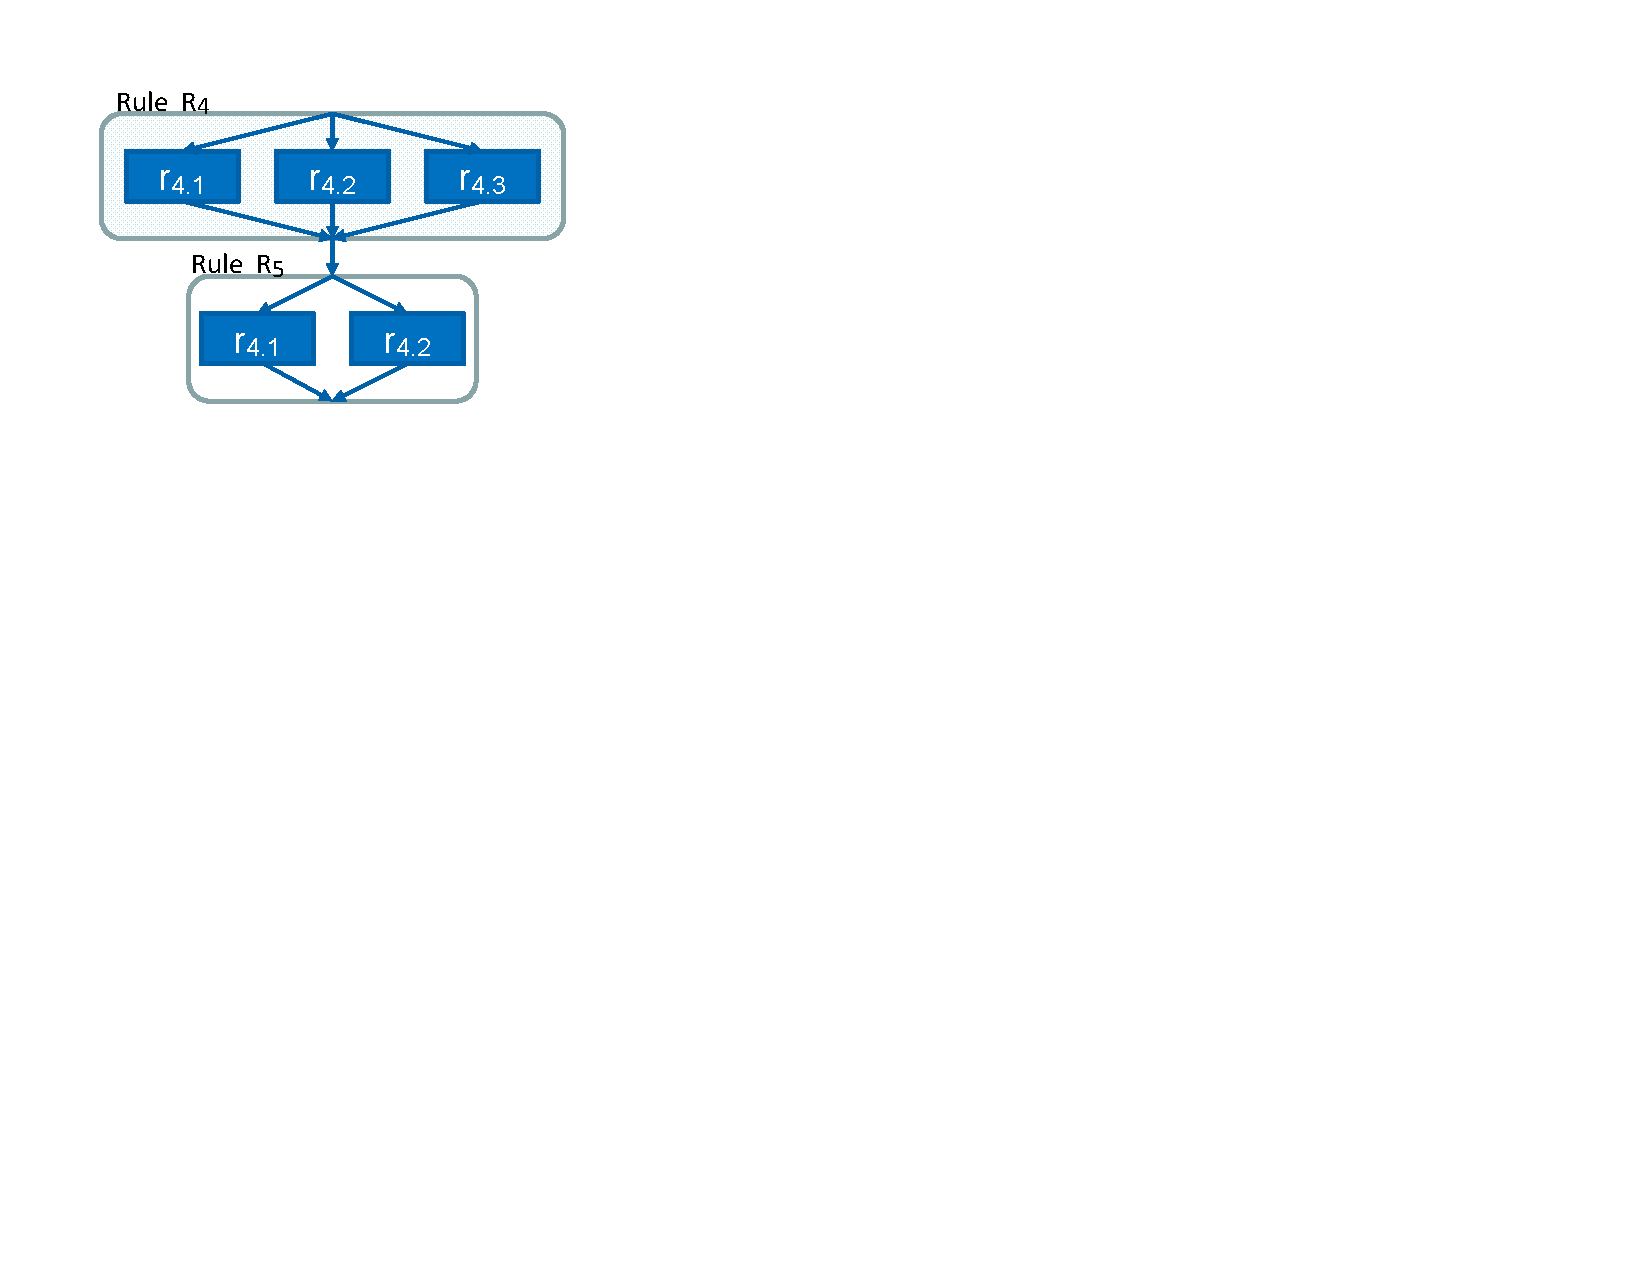
\includegraphics[trim=48 390 520 38,clip,width=2in]{figs/cfg-example.pdf}
\caption{Operation flow graph for the \subject{GenerateInvoice} operation.}
\label{fig:cfg}
\end{figure}

\begin{algorithm}[t]
\footnotesize
\SetAlgoVlined
\KwIn{Operation ${\cal O}$, Rule part $r$}
\KwOut{Concrete sequence $seq$ or $null$}
\BlankLine

\nl Let $q$ represents a queue of concrete sequences\;
\nl Generate all initialization sequences $iseqs$ for ${\cal O}$\;
\nl \ForEach {sequence $iseq \in iseqs$}
{
		\nl Generate all concrete sequences $cseqs$ for $iseq$\;
		\nl Add $cseqs$ to queue $q$\;
} 

\nl \While { q not empty }
{
		\nl Dequeue sequence $cseq$ from $q$\;
		\nl Check whether $cseq$ is satisfiable\;
		\nl \If {satisfiable}
		{
				\Return $cseq$\;
		}
		
		\nl Extract unsatisfiable core $ucore$ of $cseq$\;
		
		\nl \If {$cseq$ not helping to make progress}
		{
				{\bf continue}\;
		}
		
		\nl Identify operations $ops$ that help satisfy $ucore$\;		
		\nl \ForEach {operation $op \in ops$}
		{
			\nl Generate new sequences $nseqs$ by adding $op$ to $cseq$\;
			\nl Add all $nseqs$ to queue $q$\;
		}
}

\Return $null$\;
		
\caption{\label{alg:guidedsearch} Algorithm for
  identifying a concrete sequence that cover a given rule part.}
\end{algorithm}

\subsection{Algorithm}
\label{sec:technique}

Our algorithm accepts an operation ${\cal O}$ and a rule part $r$, and
generates a concrete sequence $seq$ that helps cover $r$. For illustration
purposes, we consider the operation ${\cal O}$ as \subject{GenerateInvoice} and 
rule part $r$ as $r_{4.2}$. For brevity,
we omit details such as exiting the main loop (lines 6-15) when user-defined
threshold of maximum number of sequences to be explored is reached.

\textit{Generate Initialization Sequences (Lines 2--5).} Given an operation ${\cal O}$, our algorithm
first generates all possible initialization sequences that produce input entities of ${\cal O}$
using dependency graph. An initialization sequence is the same as an 
abstract sequence, however, includes only those
operations that create entities. In particular, 
our algorithm first identifies input entities 
$I = \{i_1, i_2, \ldots, i_m\}$ of ${\cal O}$ through \textit{read}
edges in the graph. For each entity $i_k$, it identifies set of operations 
$OP_k = \{{\cal O}^k_1, {\cal O}^k_2, \ldots, {\cal O}^k_n\}$
that create $i_k$ through \textit{create} edges in the graph. Note that our model
allows multiple operations to create an entity. Next, our algorithm produces
combinations of all operations across each set corresponding to $i_k$ 
to generate initialization sequences. Therefore, if there are $m$ input entities
and $n$ operations that create each entity, our algorithm generates $n ^ m$
initialization sequences. Note that the order of operations 
among these sequences does not matter, since they create different entities.
Although in theory the number of initialization sequences could be high, however
in practice based on our empirical experience, we found that the number of operations
that create entities is often quite low, resulting in only a few initialization
sequences.

Next, our algorithm checks whether any operation in each $OP_i$
further requires additional entities, and repeats this process until no 
new input entities are required in all initialization sequences. 
For our illustrative example, the initialization sequence for 
the operation \subject{GenerateInvoice} is shown below.

\vspace*{-5pt}
{\small
\begin{alltt}
  State st; BalanceType bt;
  CreateCustomer(st, bt, out Customer cust);  
  CreateOrder(cust, out Order ord);
  GenerateInvoice(ord, out Invoice inv);  
\end{alltt}
}
\vspace*{-5pt}

Next, from each initialization sequence,
our algorithm generates concrete sequences by computing all possible combinations of
rule parts among operations in the sequence. To achieve this, our algorithm
joins operation flow graphs corresponding to each individual operation in the sequence and then
enumerates all paths in the final flow graph. These concrete sequences generate different
object states for input entities of the operation ${\cal O}$. For our current example,
there is only one concrete sequence, since each operation in the
preceding initialization sequence includes only one rule part.

\vspace*{-5pt}
{\small
\begin{alltt}
  State st; BalanceType bt;
  CreateCustomer(st, bt, out Customer cust) [\(r\sb{1.1}\)];
  CreateOrder(cust, out Order ord) [\(r\sb{3.1}\)];	
  GenerateInvoice(ord, out Invoice inv) [\(r\sb{4.2}\)];  
\end{alltt}
}
\vspace*{-5pt}

\textit{Check Satisfiability (Line 8).} Next, our algorithm checks whether 
concrete sequences in the queue are satisfiable. A concrete sequence 
is considered as satisfiable if it generates desired
object states for all input entities of ${\cal O}$ that help cover the precondition of the rule
part $r$. To achieve this, our algorithm constructs a logical formula composed
of constraints in preconditions and postconditions in each rule part of the sequence
and then leverages a constraint solver to check whether the composed
formula is satisfiable or not.

For illustration purposes, consider the sequence of operations and their selected
rule parts as $({\cal O}_1 [r_{1.1}], {\cal O}_2 [r_{2.1}], \ldots, {\cal O}_n [r_{n.1}], {\cal O} [r])$.
Our algorithm starts with the precondition of $r$ (referred to as $target$) in the operation ${\cal O}$. 
It next generates binding constraints that substitute the entities
consumed by ${\cal O}$ by the entities created or
modified by the predecessor operation ${\cal O}_n$. These binding constraints bind 
the identifiers in the postcondition of $r_{n.1}$ to the identifiers of the same type
in the precondition of $r$. Since the solver has no
notion of objects, our binding constraints ensure that referenced object attributes
are appropriately bound as well.

Binding constraints are generated as follows. Let $v$ be an
identifier of type $\tau$ occurring in either the creates or modifies
clause of a predecessor such as ${\cal O}_n$ and let $w$ be an identifier of the same type
occurring in the input clause of the successor such as ${\cal O}$. If $\tau$ is an enumerated or primitive type,
the only binding constraint needed is $w = v$. On the other hand, if $\tau$ is an object type, then
we must bind all attributes as well, yielding the following constraint.

$b_n$: $w = v \wedge w.f_1 = v.f_1 \wedge \ldots \wedge w.f_n = v.f_n$ 

Here, $f_1, \ldots , f_n$ are attributes of $\tau$. If any of the
attributes are of object types themselves, this process is applied
recursively on each such attribute to generate the final binding
constraint. Using binding constraints, our algorithm generates the formula as $p_{n.1} \wedge q_{n.1}
\wedge b_n \wedge p$, where $p_{n.1}$ and $q_{n.1}$ are pre- and postconditions
of the rule part $r_{n.1}$, respectively. Our algorithm leverages a 
constraint solver to check whether the composed formula is satisfiable.
If yes, it proceeds further by considering
this formula as $target$ and ${\cal O}_{n-1}$ as the predecessor operation,
and later repeats the same process with other operations in the sequence.
Once it processes all operations in the sequence and also if the formula is satisfiable,
our algorithm extracts values for variables of primitive and enumerated types
from the solver result to generate test data. 

For our running example, the solver returns that the composed formula
as unsatisfiable. The reason is that $r_{3.1}$ of \subject{CreateOrder} 
assigns zero to the attribute \subject{total} of the \subject{Order} entity, whereas the
precondition in rule part $r_{4.2}$ of \subject{GenerateInvoice} requires the value of \subject{total} 
as greater than zero.

\textit{Extract Unsatisfiable Core (Line 10).} If the composed formula is unsatisfiable,
our algorithm extracts the unsatisfiable core \subject{ucore} of the formula. An unsatisfiable core 
is a subset of the entire formula, which preserves the unsatisfiability but is simplified
compared to the original formula. This \subject{ucore} helps identify additional operations that modify attributes of entities
to produce desired object states. Section~\ref{sec:impl} presents more implementation
details of how we extract \subject{ucore} from a formula.

In our current example, our algorithm extracts 
unsatisfiable core as \subject{ord.total = 0 $\wedge$ ord.total > 0}, composed of constraints
in rule parts $r_{3.1}$ and $r_{4.2}$. For the ease
of explanation, we present Line~11 after explaining
the rest of the algorithm.

%If the unsatisfiable core is already seen for this sequence, our algorithm
%ignores the sequence. The reason is that the candidate operation that is suggested
%earlier did not help make any additional progress by resulting in the same unsatisfiable core.
%TODO: Refer to Tao's DSN paper for fitness functions.

\textit{Identify Candidate Operations (Line 12).} Since our algorithm checks satisfiability for
each operation in the sequence beginning from the last operation, when we 
extract unsatisfiable core, it contains constraints from the formula that was
composed so far and also the constraints from the last analyzed operation. First, our algorithm
discards constraints from \subject{ucore} that are contributed by the last analyzed operation.
We use notation \subject{ucore-} to represent the remaining constraints in the extracted
unsatisfied core. The key intuition in computing \subject{ucore-} is to identify candidate operations
that are compatible with \subject{ucore-} so that the composed formula can be satisfiable.
To achieve this, our algorithm first extracts entities and their attributes involved
in \subject{ucore-}. Next, it identifies candidate operations that modify those entities.
Within each such candidate operation, our algorithm identifies rule parts 
that modify desired attributes and also whose
postconditions are compatible with \subject{ucore-}, \ie{} $q \wedge b \wedge \subject{ucore-}$
is satisfiable, where $q$ and $b$ represent postcondition of selected rule part
in the candidate operation and binding constraints, respectively. 
This additional satisfiability check helps discard candidate operations that
do modify desired attributes but still does not help in identifying the desired
sequence that can help cover the rule part $r$, thereby reducing the search
space of candidate sequences.

For our illustrative example, our algorithm identifies \subject{ucore-} as \subject{ord.total > 0}.
Next, our algorithm identifies the entity as \subject{Order} and desired attribute
that needs to be modified as \subject{total}. It further analyzes all operations
that either create or modify the \subject{Order} entity and identifies two candidate operations 
as \subject{CreateOrder} and \subject{AddItemToOrder}
and rule parts as $r_{3.1}$ and $r_{7.1}$, respectively, in those operations.
Next, it discards \subject{CreateOrder}, since $q_{3.1} \wedge \subject{ucore-}$
is not satisfiable. On the other hand, since $q_{7.1} \wedge \subject{ucore-}$
is satisfiable, our algorithm selects \subject{AddItemToOrder} as a candidate 
operation.

%TODO: write about searching operations that modify parent entites as well.

\textit{Generate Alternate Sequences (Lines 13--15).} Once a candidate operation 
(along with relevant rule parts) is identified, our algorithm
checks whether it requires any additional input entities that
are not yet available in the current sequence $cseq$.
If yes, it identifies the additional operations that create necessary
entities. Next, using dependency graph, our algorithm identifies all positions in $cseq$
where the candidate operation (along with additional operations) 
can be inserted. Note that there can be multiple positions that satisfy
dependencies for inserting the candidate operation, and these different
sequences may produce different object states for input entities of ${\cal O}$.
Therefore, our algorithm may generate multiple sequences while
inserting candidate operation into $cseq$. 
Next, our algorithm generates alternate concrete sequences by inserting
candidate operation in $cseq$ in all identified positions. 
Finally, it next adds all newly generated sequences to the queue to further
analyze those sequences.

For our illustrative example, since \subject{AddItemToOrder} requires an 
additional entity \subject{Item} that is not available
in the sequence, our algorithm adds the operation \subject{CreateItem} as well
to the newly generated sequence. After creating
the new concrete sequence, our algorithm checks satisifiability of the new sequence,
where it further detects the unsatisfiable core as \subject{cust.crLimit = 0 $\wedge$ cust.crLimit > 0}. 
Our algorithm repeats the loop 6--15, and identifies the final concrete sequence that help cover rule part $r_{4.2}$ as
follows:

\vspace*{-5pt}
{\small
\begin{alltt}
  State st; BalanceType bt; int price; int crLimit;
  CreateCustomer(st, bt, out Customer cust) [\(r\sb{1.1}\)];
  AddCreditLimit(cust, crLimit, out Customer cust1) [\(r\sb{6.1}\)];
  CreateOrder(cust, out Order ord) [\(r\sb{3.1}\)];
  CreateItem(price, out Item item) [\(r\sb{2.1}\)];
  AddItemToOrder(ord, item, out Order ord1) [\(r\sb{7.1}\)];
  GenerateInvoice(ord1, out Invoice inv) [\(r\sb{4.2}\)];  
\end{alltt}
}
\vspace*{-5pt}

\textit{Check Progress (Line 11).} We next explain the significance of conditional
check in Line~11 that helps ensure that our algorithm makes progress over iterations.
While identifying candidate operations, our algorithm discards those operations that
do not help cover the target rule part $r$ (Line~12). However, in a few cases, some of the
selected operations may not help make progress and need to be discarded to efficiently
explore the state space. To ensure that the sequence $cseq$ is making progress,
our algorithm checks the following two aspects for each $cseq$.

First, our algorithm checks whether the extracted unsatisfiable core \subject{ucore}
is already seen in previous iterations related to $cseq$. If yes, it discards $cseq$
and proceeds with the other sequences in the queue. The reason is that the candidate
operation that is added to $cseq$ in its previous iteration did not help satisfy
the previous \subject{ucore}, resulting in the same \subject{ucore} in the next
iteration as well.

Second, when \subject{ucore} includes \subject{integer} variables,
our algorithm uses a fitness function to measure whether $cseq$ helps
get closer to cover the rule part $r$ or not. The first check is sufficient to deal
with variables of \subject{boolean} or \subject{enum} types but is not
sufficient to deal with the variables of {integer} type. 

We next present an
example to illustrate the issue. Consider that our model includes another
operation \subject{RemoveItemFromOrder} that removes a selected item and
decreases the value of the \subject{Total} attribute. While identifying candidate
operations, our algorithm identifies both \subject{AddItemToOrder} and
\subject{RemoveItemFromOrder}, since both these operations modify the \subject{Total}
attribute. However, \subject{RemoveItemFromOrder} does not help cover $r_{4.2}$,
since it actually decreases the value of \subject{Total}. To address this issue,
our algorithm uses a fitness function that was originally proposed in
Fitnex~\cite{xie09:fitness} to measure whether $cseq$ helps get closer
to cover the rule part or not. The key idea is to compute a fitness value
from \subject{ucore} and check whether the value is better than the fitness
value computed during the previous iteration. If yes, proceed further 
with $cseq$, otherwise discard $cseq$ and proceed with the other sequences in the queue.
